\documentclass[letterpaper,11pt]{article}
\oddsidemargin -1.0cm \textwidth 17.4cm

\usepackage[utf8]{inputenc}
\usepackage[activeacute,spanish]{babel}
\usepackage{amsfonts,setspace}
\usepackage{amsmath}
\usepackage{amssymb, amsmath, amsthm}
\usepackage{comment}
\usepackage{amssymb}
\usepackage{dsfont}
\usepackage{anysize}
\usepackage{multicol}
\usepackage{enumerate}
\usepackage{graphicx}
\usepackage[left=2cm,top=2cm,right=2cm, bottom=2cm]{geometry}
\setlength\headheight{2em} 
\usepackage{fancyhdr}
\usepackage{multicol}
\pagestyle{fancy}
\fancyhf{}


\renewcommand{\labelenumi}{\normalsize\bfseries P\arabic{enumi}.}
\renewcommand{\labelenumii}{\normalsize\bfseries (\alph{enumii})}
\renewcommand{\labelenumiii}{\normalsize\bfseries \roman{enumiii})}


\DeclareMathOperator{\sen}{sen}
\DeclareMathOperator{\senh}{senh}
\DeclareMathOperator{\arcsen}{arcsen}
\DeclareMathOperator{\tg}{tg}
\DeclareMathOperator{\arctg}{arctg}
\DeclareMathOperator{\ctg}{ctg}
\DeclareMathOperator{\dom}{Dom}
\DeclareMathOperator{\sech}{sech}
\DeclareMathOperator{\rec}{Rec}
\DeclareMathOperator{\inte}{Int}
\DeclareMathOperator{\adh}{Adh}
\DeclareMathOperator{\fr}{Fr}
\DeclareMathOperator{\Ima}{Im}
\DeclareMathOperator{\dist}{dist}
\DeclareMathOperator{\argmin}{\text{argmín}}
\let\lim=\undefined\DeclareMathOperator*{\lim}{\text{lím}}
\let\max=\undefined\DeclareMathOperator*{\max}{\text{máx}}
\let\min=\undefined\DeclareMathOperator*{\min}{\text{mín}}
\let\inf=\undefined\DeclareMathOperator*{\inf}{\text{ínf}}


\newcommand{\pint}[2]{\left< #1,#2\right>}
\newcommand{\ssi}{\Longleftrightarrow}
\newcommand{\conv}[2]{\xrightarrow[#1\to#2]{}}
\newcommand{\imp}{\Longrightarrow}
\newcommand{\pmi}{\Longleftarrow}
\newcommand{\ipartial}[2]{\dfrac{\partial #1}{\partial #2}}
\newcommand{\ider}[2]{\dfrac{d #1}{d #2}}
\newcommand{\iipartial}[2]{\dfrac{\partial^2 #1}{\partial #2^2}}
\newcommand{\iider}[2]{\dfrac{d^2 #1}{d #2^2}}
\newcommand{\ijpartial}[3]{\dfrac{\partial^2 #1}{\partial #2 \partial #3}}
\newcommand{\N}{\mathbb{N}}
\newcommand{\Z}{\mathbb{Z}}
\newcommand{\C}{\mathbb{C}}
\newcommand{\Q}{\mathbb{Q}}
\newcommand{\R}{\mathbb{R}}
\newcommand{\K}{\mathbb{K}}
\newcommand{\sol}{\textbf{\emph{Soluci\'on: }}}
\newcommand{\dem}{\textbf{\emph{Demostraci\'on: }}}
\newcommand{\aux}[4]{\Large \textbf{Clase Auxiliar N#1: #2}}
\newcommand{\pauta}[4]{\Large \textbf{Pauta #1 N#2}}
\newcommand{\enc}[3]{\Large \textbf{#1}}
\newcommand{\norm}[1]{\lVert #1\rVert }
\newcommand{\vabs}[1]{\lvert #1\rvert}

\begin{document}

\fancyhead[L]{\itshape{Facultad de Ciencias F\'isicas y Matem\'aticas}}
\fancyhead[R]{\itshape{Universidad de Chile}}

\begin{minipage}{11.5 cm}
\begin{flushleft}
\hspace*{-0.6cm}\textbf{MA2001-4 Cálculo en Varias Variables}\\
\hspace*{-0.6cm}\textbf{Profesor:} Javier Ramírez G.\\
\hspace*{-0.6cm}\textbf{Auxiliar:} Alejandro Silva C.\\

\end{flushleft}
\end{minipage}

\begin{picture}(2,3)
    \put(370,-4){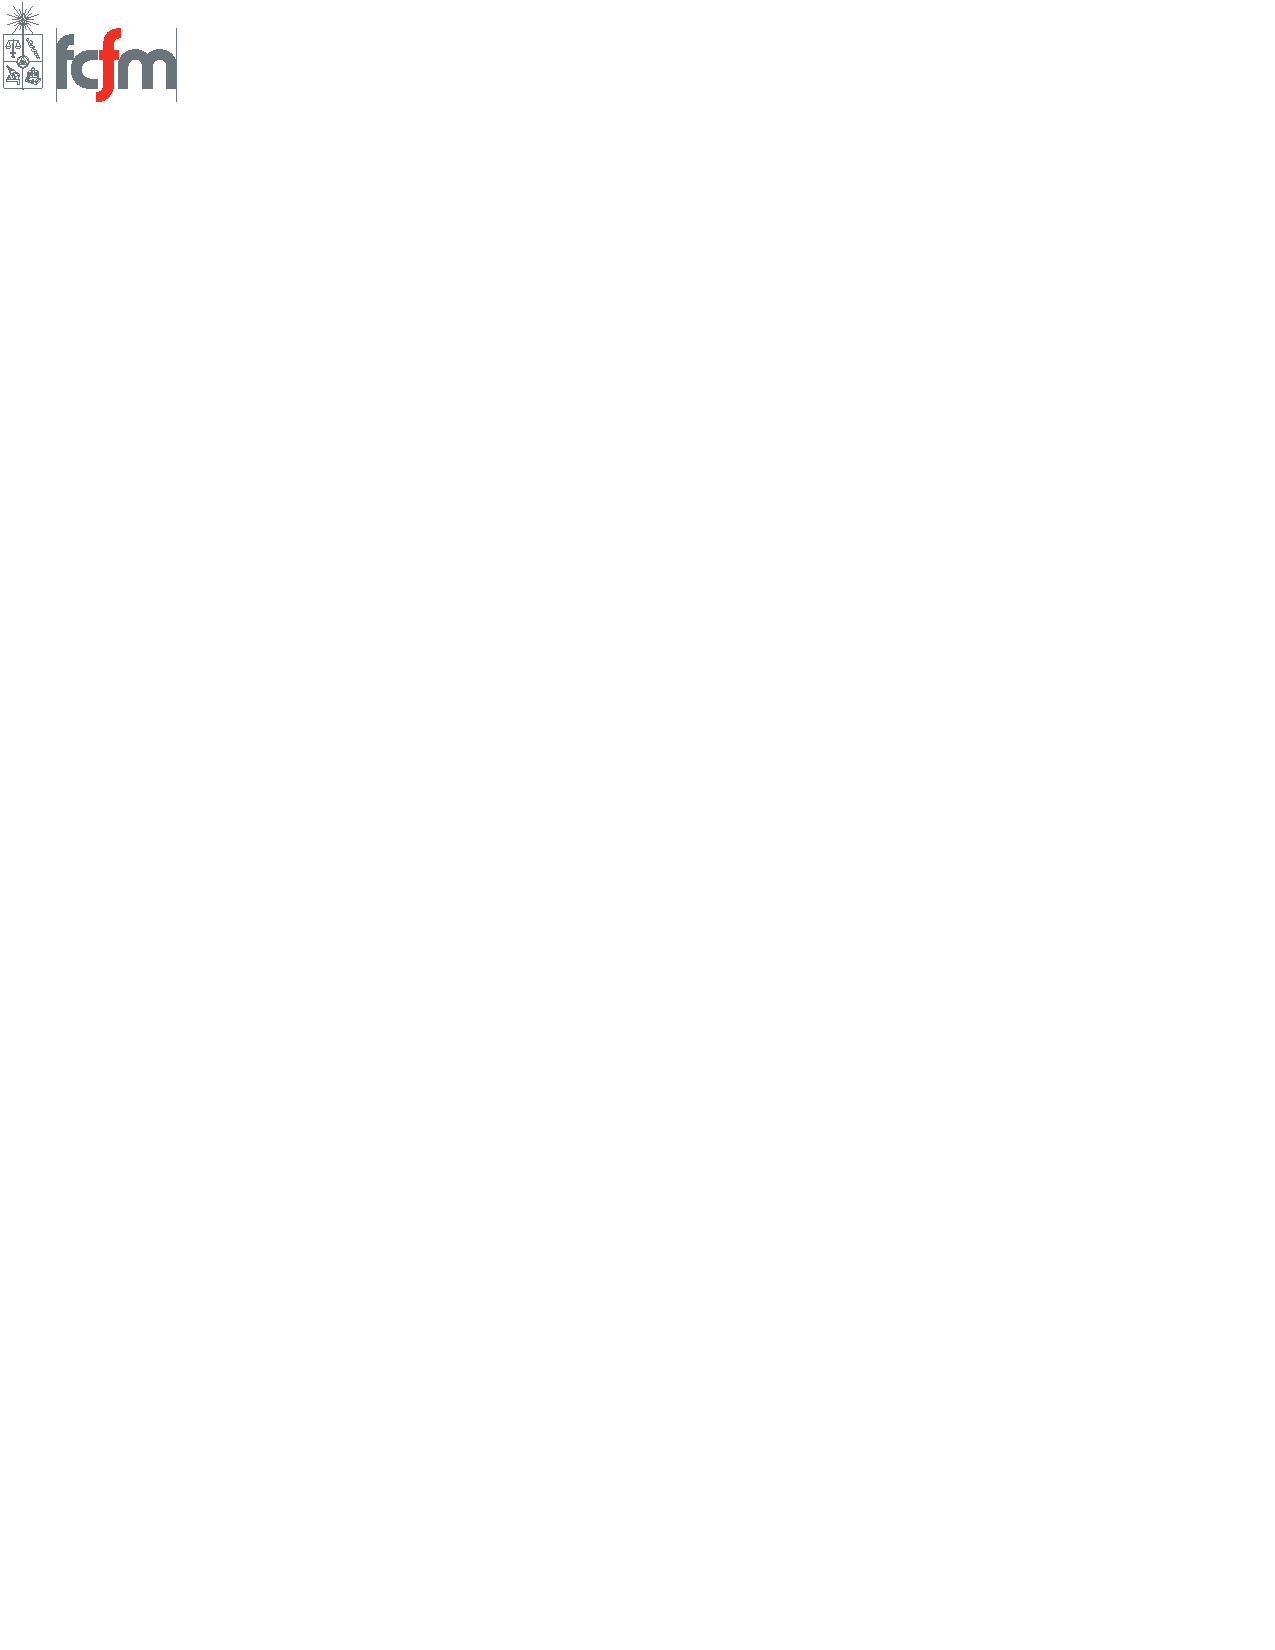
\includegraphics[scale=1.2]{fcfm2.pdf}}
\end{picture}

\begin{center}
	\LARGE \bf{Auxiliar \#9 }\\
\end{center}

\vspace{-1cm}
\begin{enumerate}\setlength{\itemsep}{0.4cm}	
\item[]

\item 
\begin{enumerate}
    \item Sea $f:\mathbb{R}^2\rightarrow \mathbb{R}$ diferenciable en todo $\mathbb{R}^2$. Se define la función $F:\mathbb{R}^2\rightarrow \mathbb{R}$ como:
    \[F(x,y)=f(f(x,y),f(x,y))\]
    Determine $\dfrac{\partial F}{\partial x}$ y $\dfrac{\partial F}{\partial y}$ en términos de $\dfrac{\partial f}{\partial x}$ y $\cfrac{\partial f}{\partial y}$
    
    \item Sean $u:\mathbb{R}^2\rightarrow\mathbb{R}$ y $v:\mathbb{R}^2\rightarrow\mathbb{R}$ dadas por:
    \begin{align*}
        u(x,y)=\dfrac{y-x}{xy}\text{,} & \quad v(y,z)=\dfrac{z-y}{yz}
    \end{align*}
    Se definen ahora $f: \mathbb{R}^2\rightarrow \mathbb{R}$, $\varphi:\mathbb{R}^3\rightarrow\mathbb{R}^2$ y $\omega:\mathbb{R}^3\rightarrow\mathbb{R}$ tal que:
    \begin{align*}
        \varphi(x,y,z)=\begin{pmatrix}
        u(x,y)\\
        v(y,z)
        \end{pmatrix} \text{,}& \quad \omega(x,y,z)=(f\circ\varphi)(x,y,z)
    \end{align*}
    Muestre que se cumple la siguiente relación:
    \[x^2\dfrac{\partial\omega}{\partial x}+y^2\dfrac{\partial\omega}{\partial y}+z^2\dfrac{\partial\omega}{\partial z}=0\]
\end{enumerate}

\item 
\begin{enumerate}
    \item Sean las funciones $g:\mathbb{R}^2\rightarrow\mathbb{R}$ y $h:\mathbb{R}^2\rightarrow\mathbb{R}$ definidas por:
    \begin{align*}
        g(x,y)=\left\{\begin{matrix}
        (x^2+y^2)sin\left(\dfrac{1}{\sqrt{x^2+y^2}}\right)&  (x,y)\neq(0,0) \\
        0 & (x,y)=(0,0) 
        \end{matrix}\right. &\qquad 
        h(x,y)=\left\{\begin{matrix}
        \dfrac{x^3-y^3}{x^2+y^2}& (x,y)\neq(0,0) \\
        0 & (x,y)=(0,0) 
        \end{matrix}\right.
    \end{align*}
    Para ambas funciones:
    \begin{enumerate}
        \item Calcule sus derivadas parciales en $(x,y)\neq(0,0)$
        \item Calcule sus derivadas direccionales, y así las parciales, en $(x,y)=(0,0)$
        \item Determine diferenciabilidad 
    \end{enumerate}
     \item Se definen $g:\mathbb{R}^2\rightarrow\mathbb{R}$ y $f:\mathbb{R}\rightarrow\mathbb{R}^2$ como:
    \begin{align*}
        g(x,y)=\left\{\begin{matrix}
    \dfrac{xy^2}{x^2+y^2} & \text{si } (x,y)\neq(0,0)\\
    0 & \text{si }(x,y)=(0,0)
    \end{matrix}\right., &\quad f(t)=\begin{pmatrix}
    at\\
    bt
    \end{pmatrix}
    \end{align*}
    En donde $a,b\in\mathbb{R}\backslash\{0\}$
    \begin{enumerate}
        \item Calcule $\dfrac{\partial g}{\partial x}$ y $\dfrac{\partial g}{\partial y}$ en $(0,0)$
        \item Determine $h=g\circ f$
        \item Calcule directamente $h^{\prime}(0)$
        \item Calcule $h^{\prime}(0)$ utilizando regla de la cadena. ¿Qué ocurrió?
    \end{enumerate}
\end{enumerate}
\end{enumerate}
\newpage
\subsection*{Problema Adicional}
\begin{enumerate}
    \item En mecánica clásica se puede determinar las ecuaciones de movimiento gracias a las ecuaciones de Euler-Lagrange definidas por:
    \[\frac{d}{dt}\left(\frac{\partial L}{\partial \dot q}\right)- \frac{\partial L}{\partial q}=0\]
    En donde $L$ es el Lagrangiano y $q$ es una coordenada generalizada. 
    
    Para un péndulo la coordenada generalizada es el ángulo entre la masa y la vertical $\theta$, y su Lagrangiano se define como:
    \[L=\frac{1}{2}mr^2{\dot\theta}^2+mgr\cos(\theta)\]
    Determine la ecuación de movimiento para el péndulo.
\end{enumerate}
\end{document}